\chapter{The Basic Laws To Maxwell's Equation (1)}\label{lec:lec18}
It was established in the previous chapter that, the origin of the electric and magnetic field is the charge. The effect of this charge is measured by a quantity called the \textbf{\emph{electric field}}. However, when the same charge is kept in motion, it constitutes a current and the presence of this current is felt by a quantity called \textbf{\emph{magnetic field}}. So we can take current as the origin of the magnetic field. 

In this chapter we will be looking at some laws like ohms law and other laws of electromagnetism and see how we can formulate these laws in mathematical form called \footnote[1]{James Clerk Maxwell, a Scottish mathematician and physicist. He was born on June 13, 1831 in Scotland and died on Nov 5, 1879 in Edinburgh. He studied electromagnetic radiation, electricity, light and gas. He is known for his formulation of electromagnetic theory and he's regarded by most modern physicists as the scientist of the 19th century who has the greatest influence on 20th century physics, for the nature of his contribution.} maxwell's equations. And also see the relationship between current and magnetic field, magnetic flux density and magnetic field.
\begin{figure}[h]
\centering
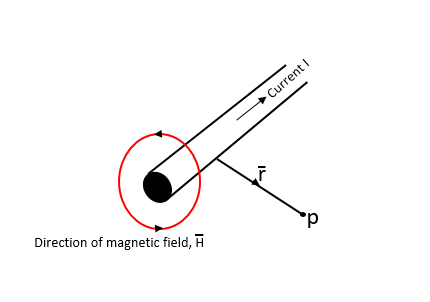
\includegraphics[height=7cm]{./graphics/currentElement}
\caption{Current carrying element(wire)}
\label{}
\end{figure}

Now let's consider a current carrying element which is a small piece of wire carrying current(I) with length given by $d\bar{l}$ having direction shown by the arrow in fig 18.1. At some point in space P given by the  distance $r$ from the current element.

The magnetic field due to the current element $Id\bar{l}$ is given by; \\
\begin{align}
\boxed{d\bar{H}= \frac{Id\bar{l} \times \hat{\textbf{r}}}{4\pi r^{2}}}\quad (Amp/m)
\end{align} 
This is the \emph{Magneto-motive force (MMF) at that point P}\index{magneto-motive force (mmf)}. Analysis From Equation 18.1
\begin{enumerate}[(i)]
\item The expression shows that the magnetic field is proportional to the current I and the length of the wire through which the current flows but inversely proportional to the square of the distance r from the current element (wire).
\item By applying right hand rule, the direction of the magnetic field ($d\bar{H}$ ) points in the clockwise direction looking in the direction of the current.
\end{enumerate}

The quantity related to the medium parameters is the magnetic flux density ($\bar{B}$) and not magnetic field ($\bar{H}$). So no matter the medium, $ d\bar{H} $ depends on I, $ d\bar{l} $ and r which are not the medium parameters. 

\section{Magnetic Flux Density $\bar{B}$}\index{magenetic flux density}
This is the product of the permeability of the medium and the magnetic field strength.\\
Mathematically, 
\begin{align}
\boxed{\bar{B} = \mu\bar{H}}\quad (Wb/m^{2})
\end{align}
Where $ \mu $ is the medium parameter called the \emph{the permeability of the medium}.

Depending upon the magnetic properties of the material, the value of permeability changes. \\
So the magnetic flux at point P, is related to the permeability of the medium and the magnetic field strength. The unit of magnetic flux density is in Tesla or $Weber/m^{2}$ . Analysis From Equation 18.2
\begin{enumerate}[(i)]
\item The magnetic flux density $\bar{B}$ tells us the density of magnetic lines of forces at that particular location. Meaning it is essentially showing you some kind of vectors which are oriented and hence the reason it is a vector quantity.
\item As we define electric field as the  \emph{force per unit charge due to presence of charges}, we can also define for magnetic field as the \emph{force experienced by a unit magnetic pole placed in the vicinity of the current}, making $\bar{B}$ and $\bar{H}$ vector quantities.
\item In the case of magnetic field, if the medium is \footnote[2]{An isotropic medium is a medium that has uniform permeability in all directions of the medium }\emph{Isotropic}, $\bar{B}$ and $\bar{H}$ will be in the same direction. Whereas if it is an \footnote[3]{Anisotropic medium is one such that the permeability and permittivity of the medium are not uniform }\emph{Anisotropic} medium $\bar{B}$ and $\bar{H}$ will not be in the same direction. The next we are looking at is Ohms law.
\end{enumerate}

\section{Ohms Law} 
We know that \footnote[4]{Ohms law was formulated by a German physicist and a mathematician, George Simon Ohm (16 March 1789 - 6 July 1854) who began as a school teacher in Brandenburg-Bayreuth, Bavaria in Germany. He attended University of Erlangen and he won Copley Medal in 1841 for his research and is known for Ohm's law, Ohm's phase law, and Ohm's acoustic law. He began his scientific career on Physics(Electricity) in univerity of Munich where Karl Christian Von Langsdorf was his Doctoral advisor.}Ohms law relating to electric field, is the relationship between voltage and current flowing in a medium or in a circuit. Ohm's law which states that the current(I) through a conductor between two points is directly proportional to the voltage(v) across the two points. However the general form of Ohm's law is the relationship between a quantity called \emph{the conduction current density $ \bar{J} $ and electric field $ \bar{E} $}.
\begin{figure}
\centering
% \includegraphics[height=5cm]{./graphics/fig182}
\caption{A conductor where the conductivity is not constant}
\label{}
\end{figure}

So if we take a medium where the conductivity of the medium is not constant, then it is not meaningful to define the total current for the medium. Normally what we do is, we define a quantity called the conduction current density $ \bar{J} $ (i.e \emph{current flowing per unit area in this conductor}). It has direction which is the direction the current is flowing. 

This current is flowing due to electric field because it has some electric potential. We have seen that the electric field is related to the gradient of potential difference.

So if we go from circuital Ohm's law, we'll have a relationship between voltage and current which have a proportional relationship and also a proportionality constant called \emph{Resistance}.

Now let's establish a relationship between the conduction current density $ \bar{J} $ and electric field $ \bar{E} $. \\
Mathematically, 
\begin{align*}
I\quad\alpha\quad V \quad\Rightarrow I = \frac{V}{R}
\end{align*} 
Making `R' subject of the formula, we have that; 
\begin{align}
R =  \frac{V}{I} 
\end{align}
\begin{center}
Where R = The introduced constant of proportionality called the resistance.
\end{center}
For a conductor of length $\ell$ and the cross sectional area `A' The resistance is directly proportional to the length and inversely proportional to the cross sectional area of the conductor. \\
Mathematically, 
\begin{align*}
R \alpha \frac{\ell}{A}\quad R = \frac{\rho\ell}{A}
\end{align*}
Substitute equation 18.3 into the above formula.We have that;
\begin{align*}
\frac{V}{I} = \frac{\rho\ell}{A}
\end{align*}
Rearranging the equation we have that; 
\begin{align}
\frac{V}{\ell} = \frac{I\rho}{A}
\end{align}
Substitute equation $\vec{E} = \frac{V}{\ell}$ into 18.4, we have that;
\begin{align*}
\vec{E} = \frac{I\rho}{A}
\end{align*}
But the ratio of current to area is given by a quantity called conduction current density J, Hence
\begin{align*}
\vec{E} = \vec{J}\rho \quad \Rightarrow \vec{J}=\frac{1}{\rho}\vec{E}
\end{align*}

Where the conductivity $ \sigma $ is the the inverse of resistivity and verse versa $ \rho $  (i.e $ \frac{1}{\rho} $ ), Hence, 
\begin{align}
\boxed{\vec{J} = \sigma \vec{E}}\quad (A/m^{2})
\end{align}
This is the \emph{Conduction current density- The general form of Ohm's law}\index{conduction current density}. Mathematically, it is the product of electric field intensity $\vec{E}$ and $\sigma$ from a reference point where $\sigma$ is the conductivity of the medium(proportionality constant).

As seen in the previous case, the relative permeability of the medium $ \mu_r $ and the conductivity of the medium $ \sigma $ (sigma) in general, could be 3 $ \times $ 3 matrix.

So if we take a medium that is isotropic, the quantity $ \mu_r$ and sigma are scalar quantities. Whereas if the media is Anisotropic such that the media property depends on the direction in general, $ \mu_r $ gets a 3$ \times $3 matrix,  and the conductivity $ \sigma $ gets a 3$ \times $3 matrix.

This is exactly the case, like we saw in the electric field where if the medium is isotropic, the direction of the displacement vector and electric field are the same. Same thing will happen in the case of magnetic field, where if the medium is isotropic, $ \bar{B}$ and $ \bar{H}$ will be in the same direction. If the medium is Anisotropic, the direction will not be the same. Some is true for conduction current density and electric field . If the medium is Anisotropic, the direction of electric and conduction current density are not the same, and $ \bar{J} $ and $\bar{E}$ are in the same direction  for isotropic medium. 

\section{The Physical Laws To Maxwell's Equation}
Now from this basic introduction of the parameters, we are set to establish the physical laws mathematically, which when compiled gives Maxwell's equation and these physical laws are the experimental verification of the postulates. There are two ways to get Maxwell's equation
\begin{enumerate}[(i)]
\item You treat it as a mathematical postulate
\item Try to represent these mathematical laws in appropriate mathematical form to give us Maxwell's equation.
\end{enumerate}

Both ways have merits, that is, if we say maxwell's equation are mathematical postulates, then they are very exact. However one could ask a question, how do you get this postulates? one cannot simply come up with these mathematical formulae, without having a background. So the background are in the physical laws. First the physical laws came by curiosity towards the relationship between electrical and magnetic field. So if we go by the picture that maxwell's equations were guided by the experimented laws, then the advantage is that we always try to see the phenomenon in physical terms. So if we have any electromagnetic phenomenon, and accept that the origin lies in the physical laws, it will always be useful to look at every phenomenon of electromagnetics physically.

However, if you treat these equations more like mathematical postulates then one may get lost in the mathematical manipulation of these equations. So from the exactness point of view, the mathematical postulates has merit, but seeing what is happening physically, first understanding the physical laws and then getting maxwell's equation.

What we will be doing in this chapter is that, we would state first the physical laws and then using the vector identities and theorems such as divergence and stokes theorems, we would try to get the mathematical form and then finally we get maxwell's equation.

\section{Gauss Law}
This law states that the total displacement(electric flux) coming out of a closed surface is equal to the net charge enclosed by the closed surface.\\
Mathematically, 
\begin{align}
\boxed{\oiint_s\bar{D}\cdot{d\bar{a}} = \iiint_v\rho dv}
\end{align}
This is  \emph{Gauss law in integral form}\index{gauss law} where $\oiint_s\bar{D}\cdot d\bar{a}$ is the total outward displacement from the total surface. Meaning using Guass' law \footnote[5]{Guass law was formulated by a German mathematician, Carl Friedrich Gauss (30 April 1777 - 23 February 1855)who developed the divergence theorem. He was the first physicist to measure  electric  and magnetic  quantities in absolute  units.He began his scientific research in university of Gottingen on mathematics and physics as his field where Johann Friedrich Ptaff and Johann Christian Martins were his doctoral advisor. He won Lalande prize in 1810 and Copley Medal in 1838. some of his own doctoral students includes Carl Wolfgang Benjamin Goldschmidt(A co-author with J.C Eduard on Analytical Optics), Johann Benedict Listing(He discovered properties of the half twisted strip in 1858, his known also by listing's law in Ophthalmology.)} to find out the total outward displacement from the total surface from the total charge integrated over the volume.
\begin{figure}[h]
\centering
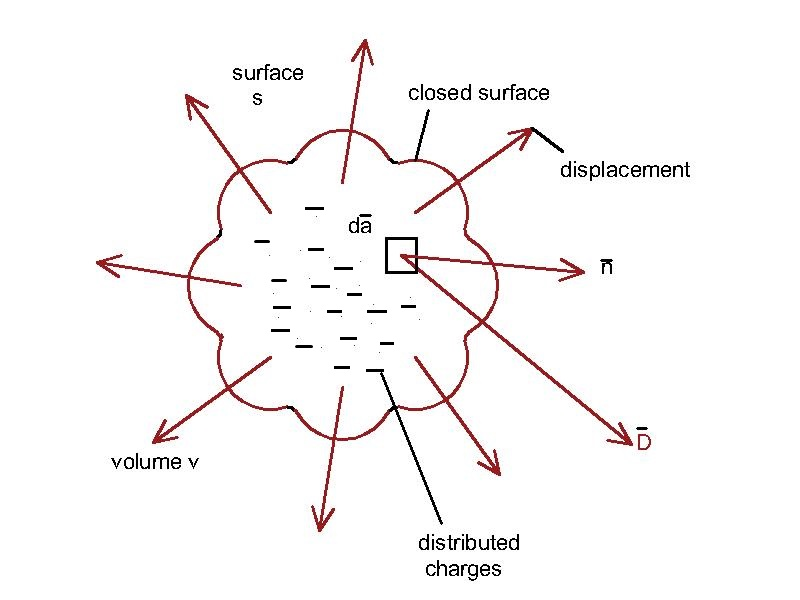
\includegraphics[height=6cm]{./graphics/g}
\caption{A closed surface showing the direction of displacement vector}
\label{fig:g}
\end{figure}

The total displacement shown by each arrow = the net charge enclosed by the surface. In general, the displacement vector will be varying as a function of the location on the surface, also it will be oriented in different directions. However the net displacement which is coming out of the surface will be the component of each arrow normal to the surface at that location.

Hence considering a small incremental area $ d\bar{a} $ on the surface as shown in figure 18.3. $ d\bar{a} $ has a direction defined by a unit normal $ \hat{n} $ with the direction of the displacement vector given by $ \bar{D} $. The outward displacement coming out from the area is the dot product of $ \bar{D} $ and $ d\bar{a} $. If that is gotten, add all the contributions from others around the surface, then we have the total displacement coming out of the close surface. Let us say in general, we have charges which are distributed inside this surface and is characterized by a charge density. This is denoted by volume charge density $ \rho $ (which is representing the density of charges inside the volume. It's S.I unit of measurement is in coulomb per cubic metres, $ C/m^{3} $).

In other words, if we add up all the charges inside the volume, we get the charge enclosed by this surface. So integrating the displacement vector over the surface, we get the total outward displacement from this surface. 
Applying\footnote[6]{$	\iint_A A\cdot d\bar{a} = \iiint (\nabla\cdot \bar{A})dv $. This is divergence law that was formulated by Guass} divergence theorem to  $\iint_s\bar{D}\cdot d\bar{a}$ (Meaning converting surface integral to line volume integral), we will have 
\begin{equation*}
\oiint_s\bar{D} \cdot d\bar{a} = \iiint_v(\nabla\cdot \bar{D})dv
\end{equation*}
\begin{equation*}
\iiint_v\rho dv = \iiint_v(\nabla\cdot \bar{D})dv
\end{equation*}
\begin{equation*}
\iiint_v(\nabla\cdot \bar{D})dv = \iiint_v\rho dv
\end{equation*}
Collect like terms and factorize out
\begin{equation*}
\iiint_v(\nabla\cdot \bar{D})dv - \iiint_v\rho dv = 0
\end{equation*}
\begin{equation*}
\iiint_v(\nabla\cdot \bar{D})dv - \iiint_v\rho dv = 0
\end{equation*}
\begin{equation*}
\iiint_v(\nabla\cdot \bar{D} - \rho)dv = 0
\end{equation*}
This relationship in the integral can only be
true for all arbitrary volume if and only if $\nabla\cdot\bar{D} - \rho = 0$
\begin{align*}
\nabla \cdot \bar{D} - \rho = 0
\end{align*}
\begin{align}
\boxed{\nabla \cdot \bar{D} = \rho}
\end{align}
Where $\bar{D}$ is the displacement vector\index{displacement vector} and $\rho$ is the volume charge density.
Analysis From Equation 18.7
\begin{enumerate}[(i)]
\item From the Gauss law in differential form, we saw that the divergence of the displacement vector at any point is related to the charge density at that point. This relationship is called point relation.
\item The differential form of Gauss law has limitation as it assumes that, we have a continuous media, meaning it will not hold for a discontinuous media (i.e the derivative at that point do not exist).
\item While the integral form of Gauss law is applicable in all situations.
\end{enumerate}
In conclusion, if the medium is continuous, we apply the differential form. But if not, we apply integral form.

Considering the relationship between the displacement vector and the electric field, we have 
\begin{align}
\boxed{\bar{D} = \epsilon\bar{E}}
\end{align}
Substituting equation 18.8 into 18.7, we have
\begin{align*}
\nabla \cdot (\epsilon\bar{E}) = \rho
\end{align*}
If we assume that the medium is homogeneous (i.e $\epsilon$ is not a function of space). Then
\begin{align} 
\boxed{\nabla \cdot \bar{E} = \frac{\rho}{\epsilon}}
\end{align} 
\emph{Gauss law for electric charges for homogeneous medium}
For a closed surface the net magnetic charge is always zero. If we apply Gauss law for the magnetic charges or poles, then there are no net charge enclosed by the closed surface. i.e
\begin{align*}
\iiint_v\rho dv = 0
\end{align*}

Hence, the net charge coming out of a closed surface for a magnetic field is always equal to zero, because there are no net magnetic charges enclosed by the surface. i.e 
\begin{align*}
\iint_s\bar{B}\cdot d\bar{a} = 0
\end{align*}
Applying divergence theorem to $\iint_s\bar{B}\cdot d\bar{a}$ we have
\begin{align*}
\iiint_v(\nabla \cdot \bar{B})dv = 0
\end{align*}	
For this to be true for any arbitrary volume $(\nabla \cdot \bar{B})$ must be equal to zero.
\begin{align}
\boxed{\nabla \cdot \bar{B} = 0}
\end{align}
\begin{center}
\emph{Gauss law for magnetic charges}
\end{center}

\section{Amperes Law}
\footnote[7]{Ampere's law was discovered by Andre Marie Ampere in 1823 }Amperes law is also called \emph{Amperes circuit law} and it states that the magneto-motive force(mmf) around a closed loop is equal to the total current enclosed by the loop.\\
Mathematically, \\
Magnetomotive Force (mmf) = $\oint_c \bar{H} \cdot d\bar{l}$ 
\begin{figure}[h]
\centering
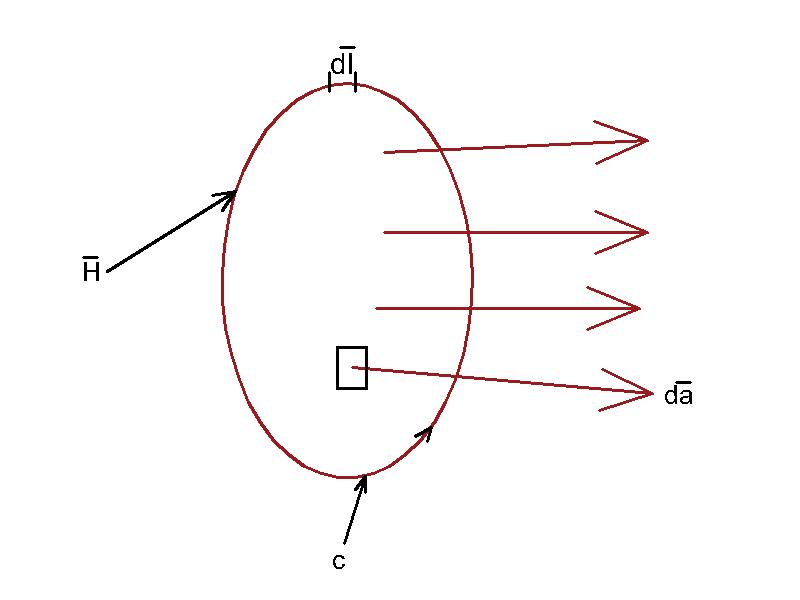
\includegraphics[height=5cm]{./graphics/j}
\caption{A loop of arbitrary size of non uniform current}
\label{fig:j}
\end{figure}

Considering a closed loop shown in fig 8.4 above, we can calculate the mmf since it is the line integral of the magnetic field along the path created by the closed loop. i.e
\begin{align*}
\Sigma I_{enclosed} &= \oint_c\bar{H}\cdot d\bar{l} = mmf
\end{align*}
Let the total current enclosed by the loop be I.\\
Therefore $\Sigma I_{enclosed} = I$
\begin{equation*}
\Rightarrow I = \oint_c\bar{H}\cdot d\bar{l}
\end{equation*}
Due to these changes, the varying current can be written as current density. The  integration of this current density $\bar{J}$ over an enclosed area created by the closed path c? gives us the total current enclosed by contour c.\\
Mathematically,
\begin{equation*}
I = \iint_A\bar{J} \cdot d\bar{a}
\end{equation*}
\begin{equation}
\boxed{\oint_c\bar{H} \cdot d\bar{l} = \iint\bar{J} \cdot d\bar{a}}
\end{equation}
This is \emph{Amperes Law in Integral Form}. Now to get the differential form of Amperes law, we will apply \emph{stroke's theorem} (i.e converting from line integral to surface integral).
\begin{equation*}
\iint_A(\nabla \times \bar{H}) \cdot d\bar{a} = \iint_A\bar{J} \cdot d\bar{a}
\end{equation*}
\begin{equation*}
\iint_A(\nabla \times \bar{H}) \cdot d\bar{a} - \iint_A\bar{J} \cdot d\bar{a} = 0
\end{equation*}
\begin{equation*}
\iint_A(\nabla \times \bar{H} - \bar{J})d\bar{a} = 0
\end{equation*} 
For this to be true for all arbitrary area, $\nabla \times \bar{H} - \bar{J}$ must be equal to zero
\begin{equation*}
\Rightarrow \nabla \times \bar{H} - \bar{J} = 0
\end{equation*}
\begin{equation}
\boxed{\nabla \times \bar{H} = \bar{J}}
\end{equation}
This is \emph{Amperes Law in Differential Form}\index{amperes law}. Analysis From Equation 18.9
\begin{enumerate}[(i)]
\item What this means is, the curl of $\bar{H}$ is equal to the total conduction current density at that point. Again the the differential form of Amperes law is only valid for a continuous medium(meaning if we go to a point and the magnetic field at that point is known(\emph{Point Relationship}), then we can apply the differential form of Amperes law). While
\item The integral form of Amperes law is applicable to the finite area enclosed by path c.
\end{enumerate}

\section{Faraday's Law of Electromagnetic Induction} 
This law states that the total Emf around a closed loop is equal to the rate of change of magnetic flux enclosed by that loop, and that, the direction of emf is such that, the magnetic field produced by this current due to this emf opposes the original magnetic field.
\begin{figure}[h]
\centering
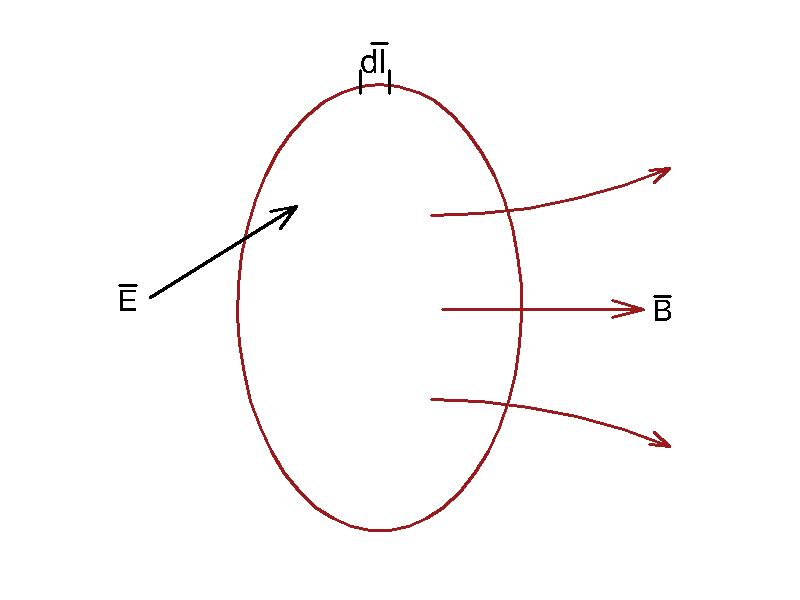
\includegraphics[height=5cm]{./graphics/k}
\caption{A closed loop used for calculating $\bar{B}$}
\label{fig:k}
\end{figure}

Considering the figure above, the total flux is found by integrating $\bar{B}$ over the area enclosed by that loop. Hence, the rate of change of this flux density is equal to the total emf produced around the loop.\\
Mathematically,
\begin{dmath}
\text{EMF} = \oint_c\bar{E} \cdot d\bar{l} = -\frac{\delta}{\delta t}(\phi)
\end{dmath}
Where $\phi$ = Total flux enclosed by the loop.
\begin{align}
\boxed{\oint_c\bar{E} \cdot d\bar{l} = -\frac{\delta}{\delta t}(\phi)}
\end{align}
This is the \emph{EMF produced by $d\bar{l}$}\index{emf}. Analysis From Equation 18.13
\begin{enumerate}[(i)]
\item The negative sign shows that the emf produced is such that, the magnetic field produced by this emf will oppose the original magnetic field. 
\item The magnetic flux can be gotten by integrating the flux density over the area created by the loop to give us the total flux. $\phi$ 
\end{enumerate}
mathematically,
\begin{align}
\phi = \iint_A\bar{B} \cdot d\bar{a}
\end{align}
Where $d\bar{a}$ = Incremental Area and $\bar{B}$ = Magnetic flux density.\\
Substituting equation 18.12 into 18.11 
\begin{align*}
\boxed{Emf = \oint_c\bar{E}\cdot d\bar{l} = -\frac{\delta}{\delta t} (\iint_A\bar{B}\cdot d\bar{a})}
\end{align*}
\emph{This is a general relationship relating to the rate of change of flux}	
\begin{align}
\boxed{\oint_c\bar{E}\cdot d\bar{l} = -\frac{\delta}{\delta t} (\iint_A\bar{B}\cdot d\bar{a})}
\end{align} 
Now let's analyze the general relationship relating the rate of change of flux.\\
The rate of change of flux can either happen in two ways.
\begin{enumerate}[(i)]
\item By varying the area of the loop with time while keeping the magnetic flux density $\bar{B}$ constant. This is called the \emph{generator action} (this is how the generator works, where the magnetic flux density is kept constant and by rotating the loop in a magnetic field, the area of the loop changes and we get induced emf).
\item By changing the magnetic flux density $\bar{B}$ with time while the area of the loop remains constant. This is called \emph{transformation action} (This is what happens in transformer where the size of the coils are not varying as the function of time, but the magnetic flux density induced in this coil vary with time which makes us have induced emf)
\end{enumerate}
Now from the integral form of Faraday's law, let's get its differential form. Hence, we are interested in the time varying fields (i.e $\bar{A}$ and $\bar{B}$ fields) and not space varying fields (loop area) which makes the area not a function of time.
\begin{align*}
{\oint_c\bar{E}\cdot d\bar{l} = -\frac{\delta}{\delta t}(\iint_A\bar{B}\cdot d\bar{a})}
\end{align*}	
Applying \footnote[9]{$\oint_c\bar{A}\cdot d\bar{l} = \iint_s(\nabla \times \bar{A})\cdot d\bar{a}$. This is original form of stokes law.}Stokes Theorem to $\oint_c\bar{E}\cdot d\bar{l}$, we have;
\begin{align*}
\oint_c\bar{E}\cdot d\bar{l} = \iint_A(\nabla\times\bar{E})\cdot d\bar{a}
\end{align*}
\begin{align*}
-\iint_A\frac{\delta \bar{B}}{\delta t}\cdot d\bar{a} = \iint_A(\nabla\times\bar{E})\cdot d\bar{a}
\end{align*}
\begin{align*}
\iint_A(\nabla\times\bar{E})\cdot d\bar{a} = -\iint_A\frac{\delta \bar{B}}{\delta t}\cdot d\bar{a}
\end{align*}
\begin{align*}
\iint_A(\nabla\times\bar{E})\cdot d\bar{a} + \iint_A\frac{\delta \bar{B}}{\delta t}\cdot d\bar{a} = 0
\end{align*}
\begin{align*}
\iint_A\{(\nabla \times \bar{E})+ \frac{\delta \bar{B}}{\delta t}\} d\bar{a} = 0
\end{align*} 
For any arbitrary area $(\nabla \times \bar{E})+ \frac{\delta \bar{B}}{\delta t}$ must be zero for the relationship to be valid.

Hence;
\begin{align*}
\nabla \times \bar{E}+ \frac{\delta \bar{B}}{\delta t} = 0
\end{align*}
\begin{align}
\nabla \times \bar{E} = -\frac{\delta \bar{B}}{\delta t}
\end{align}
This is \emph{Faraday's Law in Differential Form}\index{faraday's law}. For a time varying medium if the electric field at a particular point is known, we can find the rate of magnetic flux density at the location by finding the curl of $\bar{E}$ at that location.

For a non-time varying medium (medium whose permeability $\mu$ does not vary with time), the curl of $\bar{E}$ can give the rate of change of magnetic field strength at that location.

What that means mathematically is;\\
Recall that $\nabla \times \bar{E} = - \frac{\delta\bar{B}}{\delta t}$\\
We know that $\bar{B} = \mu \bar{H}$ $\quad$ Substituting $\bar{B}$ into the differential form of Faraday's law, we have	

\begin{align*}
\nabla \times \bar{E} = - \frac{\delta}{\delta t} (\mu\bar{H})
\end{align*}

\begin{align}	 
\nabla \times \bar{E} = -\mu\frac{\delta \bar{H}}{\delta t}
\end{align}
\emph{This is the Differential form of Faraday's Law of Electromagnetic Induction for a non-time varying medium}

\section{Summary}
\begin{enumerate}[(i)]
\item Note that the integral form of all the physical laws discussed in this chapter are applicable in all situations.

\item The origin of the electric and magnetic field is the charge. The effect of the charge is measured by a quantity called the \textbf{\emph{electric field}}.

\item Electric field can be defined as the \emph{force per unit charge due to presence of charges} 

\item When the same charge is kept in motion, it constitutes a current and the pressure of current is felt by a quantity called \textbf{\emph{magnetic field}}.

\item Magnetic field can also be defined as the \emph{force experience by a unit magnetic pole placed in the vicinity of the current}.

\item The magnetic field due to the current element $Id\bar{l}$ is given by:
$\boxed{d\bar{H}= \frac{Id\bar{l} \times \hat{\textbf{r}}}{4\pi r^{2}}}\quad (Amp/m)$ 

\item Magnetic field is proportional to the current I and the length of the wire through which the current flows, but inversely proportional to the square of the distance from the current carrying element (wire).

\item Magnetic Flux Density $\bar{B}$ is the product of the permeability of the medium and the magnetic field strength. And is given by the formula;
$$\quad\boxed{\bar{B} = \mu\bar{H}}\quad (Wb/m^{2})$$

\item The general form of Ohms law which is the relationship between conduction current density $\bar{J}$ and electric field Which given by; $\boxed{\bar{J} = \sigma\bar{E}}\quad (A/m^{2})$

\item The two ways in getting Maxwell's equation 
\begin{enumerate}[(i)]
\item	You treat it as a mathematical postulate
\item	Try to represent this mathematical laws in appropriate mathematical form to give us Maxwell's equation.
\end{enumerate}

\item Gauss law states that \emph{the total displacement coming out of a close surface is equal to the net charge enclosed by the closed surface}

\item \begin{align*}
\iint_s\bar{D}\cdot{d\bar{a}} = \iiint_v\rho dv
\end{align*}
\emph{Gauss law in integral form}

\item \begin{align*} 
\nabla \cdot \bar{E} = \frac{\rho}{\epsilon}
\end{align*} 
\emph{Gauss law for electric charges for homogeneous medium}

\item \begin{align*}
\nabla \cdot \bar{B} = 0
\end{align*}
\emph{Gauss law for magnetic charges}

\item Amperes law also called \emph{Amperes circuit law} states that the magneto-motive force(mmf) around a closed loop is equal to the total current enclosed by the loop.

\item \begin{equation*}
\oint_c\bar{H} \cdot d\bar{l} = \iint\bar{J} \cdot d\bar{a}
\end{equation*}
\emph{Amperes Law in Integral Form}

\item \begin{equation*}
\boxed{\nabla \times \bar{H} = \bar{J}}
\end{equation*}
\emph{Amperes Law in Differential Form}

\item Faraday's Law of Electromagnetic Induction states that the total Emf around a closed loop is equal to the rate of change of magnetic flux enclosed by that loop, and that, the direction of emf is such that, the magnetic field produced by this current due to this emf opposes the original magnetic field. 

\item \begin{align*}
\oint_c\bar{E} \cdot d\bar{l} = -\frac{\delta}{\delta t}(\phi)
\end{align*}
\emph{EMF produced by $d\bar{l}$}

\item The negative sign shows that the emf produced is such that, the magnetic field produced by this emf will oppose the original magnetic field. 

\item 
\begin{align*}
\nabla \times \bar{E} = -\frac{\delta \bar{B}}{\delta t}
\end{align*}
\emph{Faraday's Law in Differential Form}
\end{enumerate}

In this chapter we have seen the four basic laws (Gauss law of Electric charges, Gauss Law of Magnetic charges, The Amperes Circuit Law and Faraday Law of Electromagnetic induction) and how we were able to write each of them mathematically and in their integral and differential form using reactor algebra and theorem (Stokes's and Divergent Theorem).